\documentclass[a4paper,landscape]{article}

\usepackage{fancyhdr}
\usepackage{lastpage}
\usepackage{amsmath}
\usepackage{tikz}
\usepackage{amsfonts}
\usepackage{csvsimple}
\usepackage{graphicx}

\newcommand{\F}[2]{\ensuremath{\frac{#1}{#2}}}
\newcommand{\V}{\mathbf{}}
\newcommand{\Q}{\newpage \section*{}}
\newcommand{\LP}{\left(}
\newcommand{\RP}{\right)}

\pagestyle{fancy}
\lhead{Samuel Loomis}
\setlength{\headheight}{15pt}
\chead{Electromagnetism HW 2}
\rhead{\thepage\ of \pageref{LastPage}}
\lfoot{}
\cfoot{}
\rfoot{}

\begin{document}
\begin{landscape}

\subsection*{Question 1}
What is the bound charge distribution of an infinately long uniformly
polarized equilateral triangle whose polarization is \textbf{P}.  What
is the total bound charge? What is the far field electric field
produced by the triangle?\\

\begin{center}
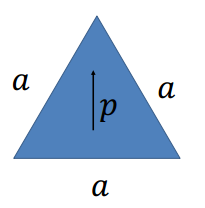
\includegraphics{Triangle-Dielectric.png}
\end{center}

Intuitively, the charge distribution will be positive pushed up, and negative pushed down.  The bottom plane of the triangle will collect the negative charges however, the top two plane will acumulate half the positive charges each.\\  The mathematical representation for the surface bound charge density is:
\[\sigma_b=\V{P}\cdot\hat{n}\]
For this triangular solid there are three normal vectors to solve for.  Measuring from $\theta=0$~pointing strait up, the three normal vectors are: $\hat{n_1}$: $\theta_1=\F{-\pi}{3}$, $\hat{n_2}$: $\theta_2=\F{\pi}{3}$, and $\hat{n_3}$: $\theta_3=\pi$.\\ \\
Solving for the surface bound charge densities:
\begin{align*}
\sigma_{b1}=\V{P}\cdot\hat{n_1}&=Pcos(\F{-\pi}{3})\\
&=\F{P}{2}\\
\sigma_{b2}=\V{P}\cdot\hat{n_2}&=Pcos(\F{\pi}{3})\\
&=\F{P}{2}\\
\sigma_{b3}=\V{P}\cdot\hat{n_3}&=Pcos(\pi)\\
&=-P\\
\end{align*}
The volume charge density is equal to the negative divergance of the polarization, and the divergance of a uniform polarization is 0, so $\rho_b$ for this material is 0.

At far distances, the minor accumulations of charge on the top and the larger acumulation of charge down below will look like a dipole.  Assuming this material extends infinitely into the page and infinitely out of the page, the electric field will only change as a funcion of theta and r, the distance away.

Another assumption to solve the field, I am going to assume that the location of the surface charges will be at the midpoints of the faces of the triangle, and the middle of the triangle is the origin.  This locates $\sigma_1$~@ (x,z) ($\F{-a}{4}$,$\F{\sqrt{3}a}{12}$), $\sigma_2$~@ ($\F{a}{4}$, $\F{\sqrt{3}a}{12}$), $\sigma_3$~@ ($0$, $\F{-\sqrt{3}a}{6}$).
\Q{Question 2}


\end{landscape}
\end{document}

